\documentclass[a4paper, 11pt]{article}
\usepackage[margin=2.2cm]{geometry}

\usepackage[utf8]{inputenc}
\usepackage[spanish]{babel}
\usepackage[babel,spanish=mexican]{csquotes}
\usepackage{hyperref}
\usepackage{graphicx}
\graphicspath{ {../img/} }
\usepackage[backend=biber,style=numeric,sorting=none]{biblatex}
\usepackage{xurl}
\addbibresource{primera-presentacion.bib}
\usepackage[table,svgnames]{xcolor}

\begin{document}

% \maketitle
\begin{center}
    \Large{\bf Uso de Redes Neuronales Convolucionales para Interpretación de Imágenes Satelitales}

    Primera Presentación - Proyecto Final de Carrera

    {
        \small

        {\bf Alumno:} Giovanni Dueck

        {\bf Tutor:} Alberto Ramírez - {\bf Cotutor:} Félix Carvallo

        Ing. Informática

        Fecha \autocite{dummy}
    }
\end{center}

\section{Introducción}

Imágenes satelitales o teledetección se refiere a imágenes capturadas por un sensor montado en un satélite artificial,
para extraer información. Estas imágenes contienen información multiespectro, es decir, además de la luz visible se
toman imágenes de bandas invisibles como por ejemplo la luz infrarroja. \autocite{globalforestlink-how-sat-imaging-work}

Para la captura de estas imágenes se emplean varios métodos, que se dividen en dos categorías: sensores pasivos
recolectan radiación electromagnética reflejada del sol, mientras que sensores activos emiten su propia radiación y
captan la reflexión de la tierra. Sensores pasivos requieren de una cantidad importante de energía para operar, pero
tienen la ventaja de operar a cualquier hora del día y la capacidad de crear imágenes en bandas que el sol no emite.
\autocite{globalforestlink-how-sat-imaging-work}

Diferentes suelos, vegetación, o humedad reflejan diferentes bandas de radiación. Estas imágenes son usadas en varias
aplicaciones, desde Sistemas de Información Geográfica y mapas a meteorología y monitoreamiento de la salud de
vegetación forestal. Un índice bastante común es el Índice de Vegetación de Diferencia Normalizada, o NDVI por sus
siglas en inglés, el cual es usado para estimar la cantidad, calidad y desarrollo de la vegetación con base a la
mediación. Estos datos ya se usan en sistemas de advertencia temprana de sequías y la predicción del rendimiento de la
agricultura en los Estados Unidos a partir de los datos de la NASA. \autocite{earthdata-vegetation}

La importancia de la producción agropecuaria y agroganadera en el Paraguay también invita a considerar estas
tecnologías para el monitoreamiento de la salud de la vegetación y el uso adecuado de la tierra. Actualmente, ya es
están empleando tecnologías de teledetección y el NDVI en el sector agrícola en aplicaciones como la detección de
malezas y predicción del orden ideal de cosecha de campos cultivados. \autocite{onesoil-agricultura-paraguay}

Con aproximadamente la mitad del territorio paraguayo hacia el norte del Río Paraguay en la región semi-árida del
Chaco, tecnologías que alivien las sequías y precipitación baja son muy valiosas, tanto para la agricultura y ganadería
en las estancias chaqueñas como para centros poblacionales más aislados como por ejemplo las comunidades indígenas.
Estos pueblos están aislados y generalamente se caracterizan por la probreza manifestada en una salud deteriorada
producto de la deficitaria alimentación y agua potable.

Un paleocauce es un cauce por el cual antiguamente fluía agua, como por ejemplo un antiguo lecho de un río. Los
paleocauces han sido propuestos como reservorios o conductos para el flujo subterráneo de agua dulce. Se consideran de
interés principalmente los paleocauces arenosos, y estos pueden ser aprovechados para acceder al agua en áreas en las
que la distribución habitual del agua no existe o está dificultada de alguna forma. \autocite{wikipedia-paleochannel}
Con la abundancia de paleocauces en el Chaco central (ocupan un 15\% de la región), esta propuesta es una bastante
prometedora que ya ha sido considerada en investigaciones anteriores. \autocite{conacyt-sistemas-captacion-agua}

La detección de estos paleocauces se haría a partir de imágenes satelitales en una serie temporal por medio de redes
neuronales. Las redes convolucionales son una categoría de redes neuronales especializadas para el procesamiento de
imágenes. El principio básico de su funcionamiento consiste en la convolución de grupos píxeles cercanos, una operación
que permite tener en cuenta no solo el valor de cada píxel individual, sino el contexto de los mismos.
\autocite{axiv-cnn-satellite-imaging}

El resto del escrito está compuesto por las siguientes secciones: (2) una breve descripción del proyecto, (3) los
objetivos general y específicos, (4) las bases conceptuales del proyecto, (5) el estado del arte relacionado al
proyecto, (6) la metodología de la solución, (7) la importancia del presente proyecto, y finalmente (8) se presenta el
estado actual del proyecto.



\section{Descripción del proyecto}

La motivación principal del proyecto es la necesidad de mitigar las sequías prolongadas del Chaco Paraguayo, que
impacta de forma más severa a zonas remotas o rurales. El objetivo del trabajo es aplicar técnicas de clasificación e
interpretación de imágenes satelitales por medio de redes neuronales al problema de la identificación de usos de suelo,
particularmente para identificar paleocauces.


\section{OBJETIVOS}

\subsection{Objetivo General}

Creación de modelos a partir de redes neuronales convolucionales para la clasificación y caracterización de imágenes satelitales.

\subsection{Objetivos Específicos}

\begin{enumerate}
    \item Análisis de series temporales a partir de imágenes satelitales correspondientes a la región occidental del Paraguay
    \item Identificación y clasificación de componentes de uso de suelo
    \item Determinación de áreas de ocurrencia de paleocauces
\end{enumerate}


\section{Marco Conceptual}

En esta sección se exploran brevemente los conceptos más fundamentales para el proyecto. En particular, los temas a
desarrollarse son una revisión del estado de la teledetección y los recursos disponibles, las bases de las redes
neuronales convolucionales y su uso en el análisis de imágenes satelitales, las técnicas modernas en uso en la
investigación y en aplicaciones en el mundo real.

\subsection{Teledetección}

Teledetección se refiere a la captación o detección remota de alguna señal o imagen. En este contexto nos referimos
específicamente a imágenes captadas por medio de un sensor montado en un satélite artificial o algún vehículo aéreo
como un avión o un dron, para extraer información. Estas imágenes contienen información multiespectro, es decir, además
de la luz visible se toman imágenes de bandas invisibles como por ejemplo la luz infrarroja.
\autocite{globalforestlink-how-sat-imaging-work} A lo largo de este proyecto, el término \enquote{teledetección} se
refiere a la captación de imágenes por medio de satélites.

Para la captura de estas imágenes se emplean varios métodos, que se dividen en dos categorías: sensores pasivos
recolectan radiación electromagnética reflejada del sol, mientras que sensores activos emiten su propia radiación y
captan la reflexión de la tierra. Sensores pasivos requieren de una cantidad importante de energía para operar, pero
tienen la ventaja de operar a cualquier hora del día y la capacidad de crear imágenes en bandas que el sol no emite.
\autocite{globalforestlink-how-sat-imaging-work}

Los primeros programas de observación de la tierra por medio de satélites surgieron en los años 70 y 80. El primero fue
el programa Landsat de los Estados Unidos en 1972, y le siguieron programas similares en India, Francia y la Unión
Europea. \autocite{esa-space-year-2007}

\begin{figure}
    \centering
    \subfloat[\centering Cámara digital normal]{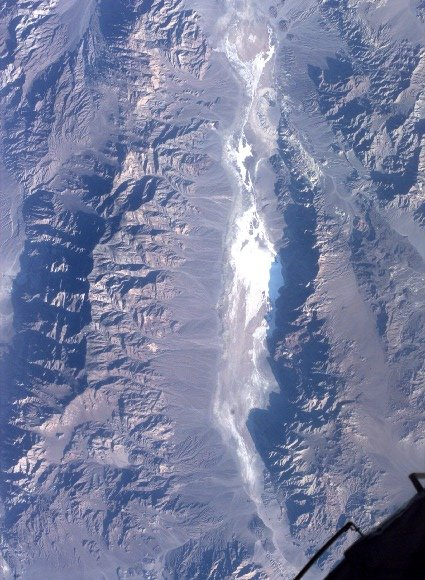
\includegraphics[width=0.275\textwidth]{img/Death_Valley_from_space.JPG}}
    \qquad
    \subfloat[\centering Radar de Apertura Sintética]{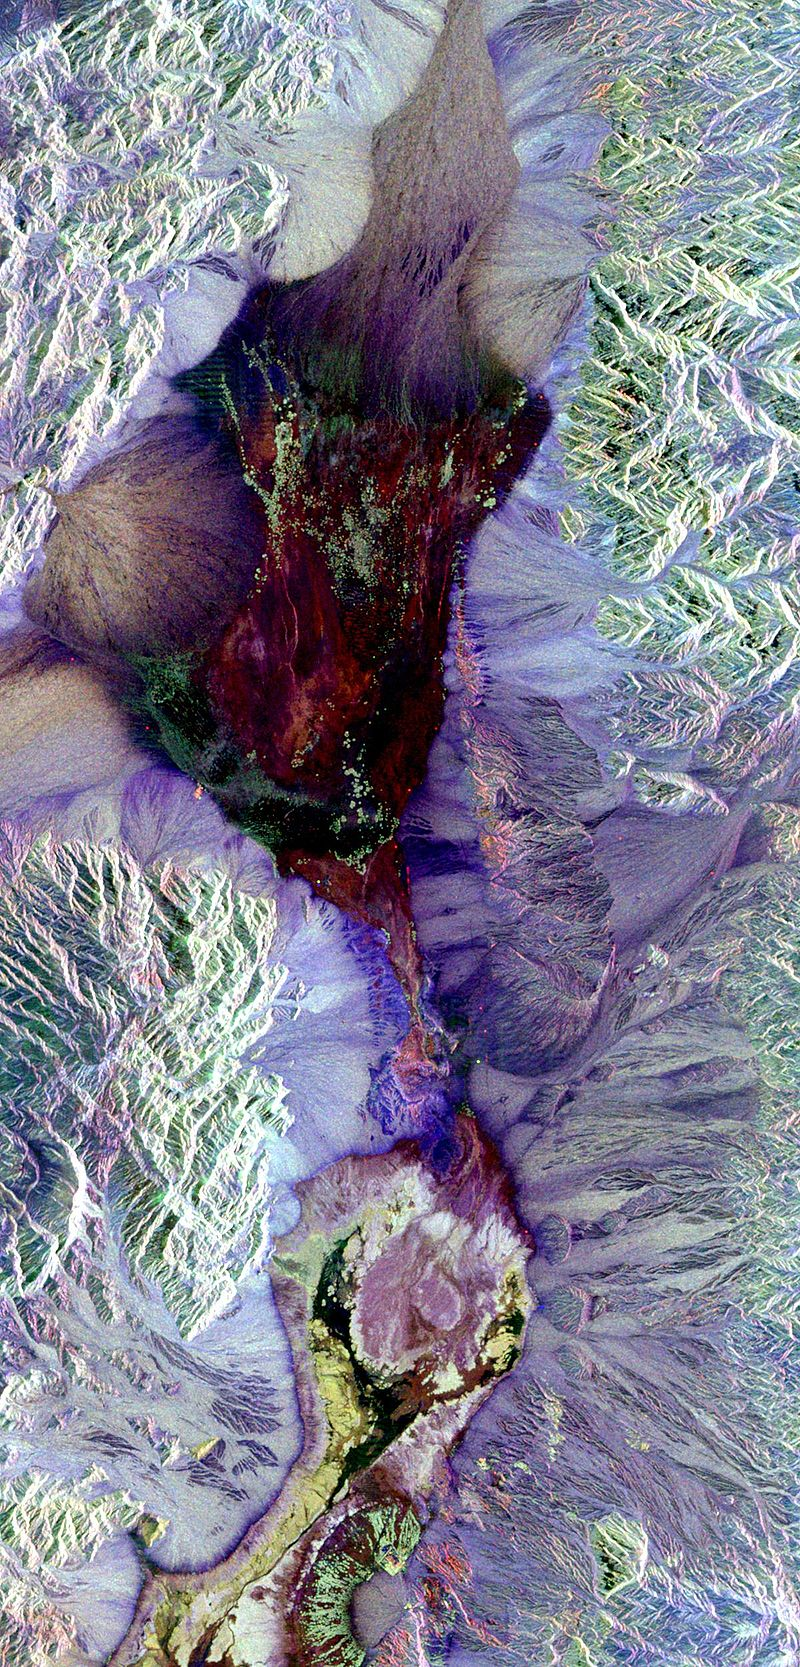
\includegraphics[width=0.175\textwidth]{img/800px-Death-valley-sar.jpg}}
    \caption{Imágenes satelitales del Valle de la Muerte con diferentes resoluciones espectrales. El área superior de (a)
    coincide con el área inferior de (b).}
    \label{fig:1}
\end{figure}

\subsubsection{Aplicaciones}

Imágenes satelitales proveen información muy útil para todo tipo de estadísticas en áreas relacionadas con el
territorio, como por ejemplo la agricultura, silvicultura y el estudio de uso del suelo. El estudio de la agricultura a
gran escala por medio de la teledetección se realizó por primera vez entre 1974 y 1977 por medio de datos de Landsat 1,
a cargo de la NASA, la Oficina Nacional de Administración Oceánica y Atmosférica (NOAA) y el Departamento de
Agricultura de los Estados Unidos (USDA). \autocite{allen-usda-study}

Dado que las imágenes producidas generalmente cubren toda o casi toda el área de estudio, y que suelen ser
multiespectrales, lo que provee datos que fotografías ordinarias no contienen, cualquier aplicación que involucre
estudiar un área vasta puede beneficiarse de ellas. Dependiendo de la resolución, aplicaciones que involucren detalles
más finos también las pueden aprovechar, como por ejemplo su uso en aplicaciones de mapas digitales.

\subsubsection{Características de los datos}

La calidad de imágenes recolectadas por teledetección se mide de cuatro formas, estas son su resolución espacial,
espectral, radiométrica y temporal.

{\bf Resolución espacial}: el tamaño de un píxel en una imagen rasterizada. Típicamente corresponde a un área cuadrada
de entre 1 y 1000 $m^2$.

{\bf Resolución espectral}: la longitud de onda de las diferentes bandas de frecuencia capturadas, normalmente
relacionada a la cantidad de bandas de frecuencia. El sensor Hyperion en \enquote{Earth Observing-1}, por ejemplo,
observa 220 bandas entre 0,4 y 2,5 $\mu m$, con una resolución espectral de 0,10--1.11 $\mu m$ por
banda. \autocite{earth-observatory-earth-observing-1} En imágenes de espectros no visibles, la visualización se hace
con colores falsos, en donde cada banda es asignada un color visible. Un ejemplo se ve en la figura \ref{fig:1}.

{\bf Resolución radiométrica}: la cantidad de niveles de intensidad de radiación detectable por el sensor. Típicamente
entre 8 y 14 bits de información, correspondiente a 256 a 16384 niveles en cada banda. La cantidad de ruido en el
sensor también afecta la resolución radiométrica.

{\bf Resolución temporal}: la cantidad de sobrevuelos del avión o satélite, importante solamente cuando se realizan
series de tiempo, promedios o mosaicos, como por ejemplo en el monitoreamiento de la agricultura.

\begin{figure}
    \centering
    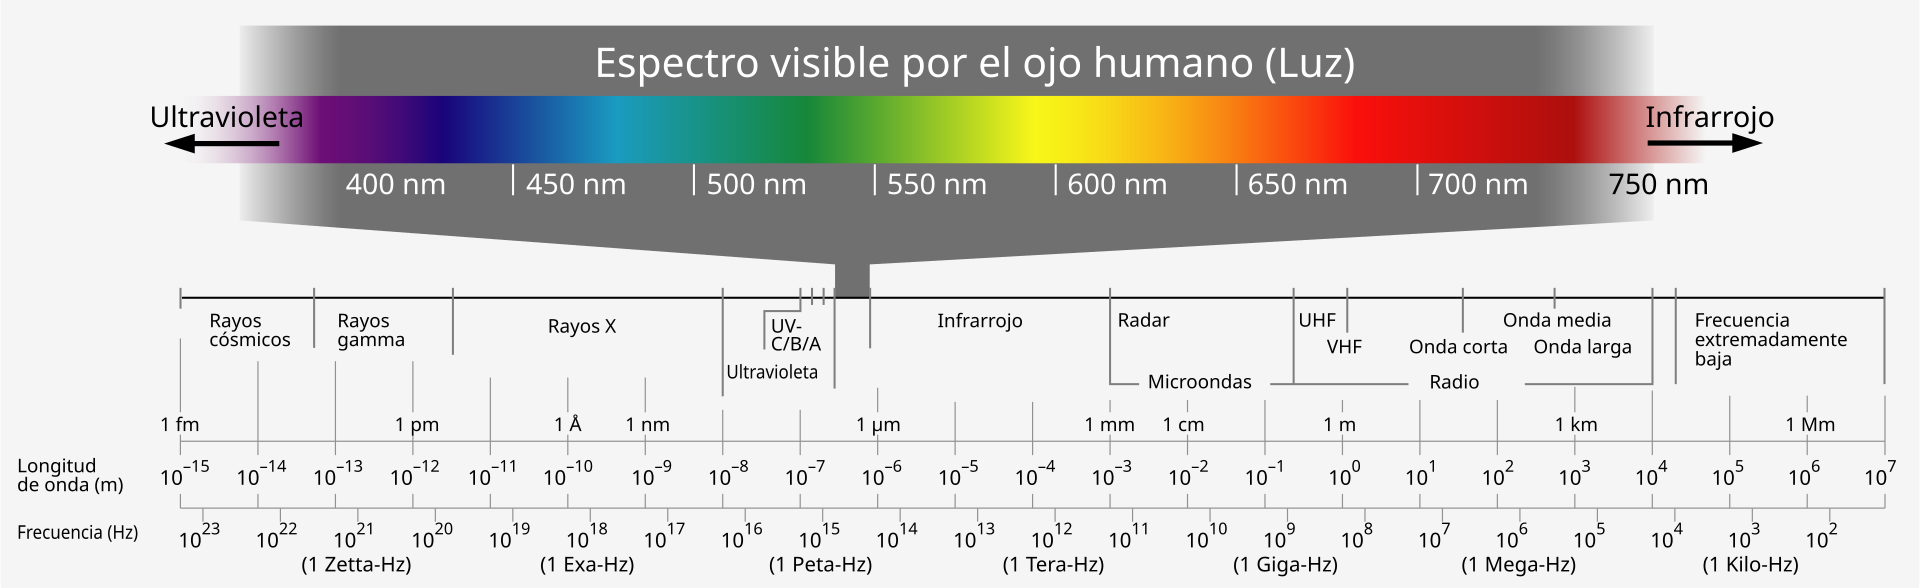
\includegraphics[width=0.9\textwidth]{img/Electromagnetic_spectrum-es.svg.png}
    \caption{Espectro electromagnético visualizado. Diferentes sustancias y materiales reflejan una variedad de
    frecuencias más allá del espectro visible, que es relativamente reducido.}
    \label{fig:3}
\end{figure}

\subsubsection{Disponibilidad de recursos}

Existen varios repositorios de datos de teledetección disponibles para usos comerciales como académicos. Los programas
de observación terrestre de la NASA y de la ESA, Landsat y Copernicus respectivamente, disponibilizan recursos por
medio de portales en la internet. Para los datos de Landsat, uno de los recursos más accesibles es Google Earth Engine,
que permite el procesamiento de imágenes en línea, de forma gratuita para usos no comerciales.
\autocite{landsat-data-access} El programa Copernicus por otro lado provee un navegador de imágenes, una forma de
descargar datos con algunos filtros, y todo esto de forma gratuita tanto para fines académicos como comerciales.
\autocite{copernicus-licences} También ofrecen un espacio de trabajo en línea, similar en propósito a Google Earth
Engine. \autocite{copernicus-ds-about}


\subsection{Redes Neuronales Convolucionales}

Una Red Neuronal Convolucional (o CNN por sus siglas en inglés) es un tipo de red neuronal artificial en la cual las
neuronas procesan datos de entrada por medio de filtros de convolución. Esto implica el procesamiento de un grupo de
datos cercanos, lo que permite interpretar el contexto de un dato, en contraste con redes neuronales típicas. Esta
propiedad hace que las CNN sean el método preferido para el procesamiento de imágenes por medio de redes neuronales.
\autocite{hands-on-machine-learning} \autocite{ciresan-cnn}

Este método de procesamiento permite procesar una gran cantidad de entradas con una cantidad reducida de neuronas,
comparado con una red neuronal típica con la misma capacidad.

Por ejemplo, considerando una red neuronal con una capa de entrada y una capa siguiente con la misma cantidad de
neuronas $N$ en ambas, una red neuronal densa, es decir donde cada neurona de una capa está conectada a cada neurona de
la siguiente capa, contiene $N \times N$ conexiones. En contraste, una red neuronal convolucional equivalente estaría
compuesta de tan solo $N$ neuronas, mientras que al mismo tiempo captura un grupo de píxeles en cada neurona en lugar
de uno solo.

Para el procesamiento se utilizan los filtros de convolución, matrices de dimensiones reducidas comparadas con la
imagen, cuyas celdas contienen coeficientes. Este filtro se superpone sobre una sección de la imagen, y los valores de
los píxeles se multiplican con los de la celda superpuesta del filtro, y la suma de los productos es el resultado de la
convolución del grupo de píxeles. Con una representación adecuada de los datos de cada píxel, estos filtros, también
llamados {\it kernels }, pueden usarse en la detección de bordes en cualquier orientación, reducción de ruido,
aumentación de intensidad de píxeles de cierto color o brillo, entre otros. \autocite{ciresan-cnn}

\subsubsection{Aplicaciones}

CNN ya se han utilizado en todo tipo de aplicaciones relacionadas con imágenes y videos, entre ellas clasificación de
imágenes, segmentación de imágenes, detección de objetos e inclusive en análisis de imágenes de inundación para
predecir la gravedad de uno de estos tipos de desastre natural. \autocite{pally2022105285}

También se ha usado extensivamente en aplicaciones relacionadas a la teledetección, con una gran colección de técnicas,
conjuntos de datos, material de aprendizaje y software de libre acceso en artículos web, videos y repositorios de
código. \autocite{tds-landuse-classification} \autocite{repo-satellite-image-dl} Queda claro que los modelos
convolucionales son muy eficaces en el procesamiento de imágenes, y la cantidad de material estudiado relacionado a las
imágenes satelitales facilitaría enormemente la aplicación en el tema de este proyecto.

\subsubsection{Técnicas y arquitecturas}


\subsection{Análisis de imágenes satelitales}

Las formas más comunes de análisis de imágenes son la clasificación, la segmentación, la detección de cambios y las
series de tiempo. Existen muchas técnicas usadas en aplicaciones más específicas, como la predicción del rendimiento de
una plantación o la salud de la vegetación, la reducción de ruido o redes generativas, que no se aplican tan
directamente para el objetivo de este trabajo.

\subsubsection{Clasificación}

La clasificación es una tarea fundamental en el análisis de datos de teledetección, en el cual el objetivo es etiquetar
cada imagen, como por ejemplo \enquote{área urbana}, \enquote{bosque}, \enquote{agricultura}, etc. El proceso de
asignar etiquetas a imágenes se conoce como clasificación a nivel de imagen. \autocite{repo-satellite-image-dl}

Sin embargo, en algunos casos una imagen puede contener más de un tipo de uso de suelo, como por ejemplo un bosque con
un río que lo divide, o una ciudad con áreas comerciales y residenciales. En estos casos, clasificación a nivel de
imagen se vuelve más compleja e invuelve asignar múltiples etiquetas a cada imagen. Esto se puede lograr por medio de
una combinación de extracción de características y algoritmos de {\it machine learning} para identificar los diferentes
tipos de uso de suelo. \autocite{repo-satellite-image-dl}

Es importante no confundir la clasificación a nivel de imagen con la clasificación a nivel de píxel, también conocida
como segmentación semántica. Mientras que clasificación a nivel de imagen asigna una etiqueta a una imagen entera, la
segmentación semántica asigna una etiqueta a cada píxel de la imagen, lo que resulta en una representación detallada y
precisa del uso de suelo en una imagen. \autocite{cole-segmentation}

\subsubsection{Segmentación}

La segmentación consiste en dividir una imagen en segmentos o regiones semánticamente significativas. El proceso de
segmentación de imágenes asigna una etiqueta de clase a cada píxel de una imagen, transformándola de una grilla 2D de
píxeles a una grilla 2D de etiquetas. Una aplicación común es la segmentación de calles o edificios, donde el objetivo
es separar las calles y los edificios de otras características de la imagen. \autocite{repo-satellite-image-dl}

Para realizar esta tarea, modelos de una clase única son frecuentemente entrenados para detectar y diferenciar entre
calles y el ambiente, o edificios y el ambiente. Estos modelos se diseñan para reconocer características específicas
como el color, la textura y la forma que son típicas de una calle o un edificio para que puedan etiquetar los píxeles
que forman parte de estas estructuras en una imagen. \autocite{cole-segmentation}

Otras aplicaciones comunes se encuentran en la agricultura o clasificación de uso de suelo en una imagen. En este caso,
se utilizan modelos multiclase que son capaces de diferenciar entre varias clases en una imagen, como por ejemplo
bosques, áreas urbanas y tierra agrícola. Estos modelos son capaces de reconocer relaciones más complejas entre tipos
de uso de suelo, y permiten un entendimiento más integral del contenido de la imagen. \autocite{cole-segmentation}



\section{Estado del Arte}

En este capítulo se explora el estado del arte del uso de imágenes satelitales en diversas áreas y las técnicas de
análisis relevantes para este proyecto. Esta investigación tiene el fin de entender la forma en que se aplican en sus
diversos campos de aplicación y cuáles técnicas son las más eficaces en el campo a estudiarse.

\subsection{Estrategias de búsqueda}

Para la revisión de literatura se utilizaron términos referentes a [Redes Neuronales], [Teledetección], y
[Clasificación y Detección]. Se tuvieron en cuenta principalmente obras en el idioma inglés, aunque se incluyen obras
en español también. Para la búsqueda se uaron los siguientes términos:

\begin{center}
    \begin{tabular}{ l | l }
        {\bf Términos } & {\bf Sinónimos } \\
        \hline
        Neural Network & Convolutional Neural Network \\
                       & Deep Learning \\
        \hline
        Remote Sensing & Satellite Imagery \\
        \hline
        Classification & Detection \\
        \hline
        Lack of data & Small data \\
    \end{tabular}
\end{center}

Las cadenas de búsqueda se construyen a partir de los términos y sus sinónimos. Las cadenas con mejores resultados
fueron
[{\it Neural Network AND Remote Sensing AND Classification }],
[{\it Convolutional Neural Network AND Remote Sensing AND Classification }],
[{\it Convolutional Neural Network AND Satellite Imagery AND Classification }],
[{\it Convolutional Neural Network AND Satellite Imagery AND Detection }], y
[{\it Deep Learning AND Remote Sensing AND Small Data }]

El motor de búsqueda utilizado fue Google Scholar, poniendo mayor enfoque en resultados provinientes de bases de datos
reconocidas y establecidas como IEEE Xplore, ScienceDirect y ArXiv.

{\bf Criterios de selección} Se incluyen artículos, papers, conferencias, y otros trabajos formales debidamente
documentados. Se establecen los siguientes criterios para juzgar si un trabajo es incluído o excluído de esta
investigación:
\begin{itemize}
    \item[] {\bf Inclusión 1} Trabajos que se enfoquen en la clasificación de imágenes satelitales por medio de redes
        neuronales en el rango de publicación de 2014 a 2024.
    \item[] {\bf Inclusión 2} Trabajos que coincidan en su contenido con los términos de búsqueda.
    \item[] {\bf Inclusión 3} Trabajos cuyo contenido sea relevante para la investigación.
    \item[] {\bf Exclusión 1} Trabajos que no contengan las palabras claves o son irrelevantes para el campo de
        investigación.
    \item[] {\bf Exclusión 2} Trabajos que se centran en un término de busqueda pero no incluyen alguno de los demás.
    \item[] {\bf Exclusión 3} Trabajos con una cantidad mayoritaria de información irrelevante para el tema estudiado.
\end{itemize}

{\bf Procedimientos de selección} El proceso de selección de trabajos se basa en responder las preguntas de
investigación presentadas en la siguiente sección, con el fin de responderlas con información válida y actual.

Se limita el número de artículos incluídos a 20, y en caso de que se supere la cantidad encontrada se filtran por medio
de los siguientes criterios:

\begin{itemize}
    \item[] {\bf P.S.1.} Los trabajos deben responder la mayor cantidad de preguntas de investigación.
    \item[] {\bf P.S.2.} Los trabajos deben contar con la mayor cantidad de incidencia de términos definidos
        anteriormente.
    \item[] {\bf P.S.3.} Artículos que incluyan las palabras clasificar, interpretar, imágenes satelitales, redes
        neuronales, redes neuronales convolucionales en su resumen, conclusión.
\end{itemize}

{\bf Extracción y síntesis de datos} Para la planilla de extracción de datos de cada estudio, se guardaron título,
autores, año de publicación, resumen, palabras claves, fuente y conclusiones relacionadas a las preguntas de
investigación. En el cuadro de la sección de resultados se listan las informaciones relevantes para responder las
preguntas de investigación de este proyecto. Para determinar la inclusión de cada artículo se realizó un análisis de
los objetivos y resultados de cada trabajo, teniendo en cuenta los criterios de selección. Para realizar la síntesis de
los datos se realizó la estrategia descriptiva, que detalla y ordena las conclusiones principales de los autores de los
artículos para una mejor compresión de las ideas principales.

\subsection{Preguntas de investigación}

El objetivo principal de este estudio es determinar cual es el estado del arte en técnicas utilizadas para clasificar y
caracterizar o interpretar imágenes satelitales por medio de redes neuronales convolucionales. Con este fin en mente,
se plantean las siguientes preguntas de investigación:

\begin{enumerate}
    \item[] {\bf P.1.} ¿Qué proyectos se están llevando adelante para clasificar y caracterizar imágenes satelitales
        usando redes neuronales convolucionales?
    \item[] {\bf P.2.} ¿Cuáles son las ventajas y/o desventajas de la clasificación y caracterización de imágenes
        satelitales usando redes neuronales convolucionales en comparación con las alternativas?
    \item[] {\bf P.3.} ¿Qué soluciones existen para abordar la falta de datos de entrenamiento para las redes
        neuronales convolucionales?
\end{enumerate}

\subsection{Resultados}

\begin{center}
    \begin{table}[h]
        \small
        \begin{tabular}{|c|c|c|c|}
            \hline
            \bf Proyecto & \bf Objetivos & \bf Métodos & \bf Observaciones \\
            \hline
            \autocite{langkvist-2016} & & & \\
            \hline
            \autocite{luengo-2016} & & & \\
            \hline
            \autocite{maggiori-2016-1} & & & \\
            \hline
            \autocite{sevo-2016} & & & \\
            \hline
            \autocite{zhong-2016} & & & \\
            \hline
            \autocite{sharma-2017} & & & \\
            \hline
            \autocite{pritt-2018} & & & \\
            \hline
            \autocite{rezaee-2018} & & & \\
            \hline
            \autocite{liu-2019} & & & \\
            \hline
            \autocite{amato-2023} & & & \\
            \hline
        \end{tabular}
        \caption{Algunos proyectos de clasificación de imágenes de teledetección por medio de CNN}
        \label{table:1}
    \end{table}
\end{center}

\begin{center}
    \begin{table}[h]
        \begin{tabular}{ |c|m{11cm}|c| }
            \hline
            \bf Tipo & \bf Característica & \bf Referencias \\
            \hline
            Ventaja & CNN patch-based (basado en pedazos) mejor que NN convencional o CNN basados en pixeles, SVN o RF
                    & \autocite{sharma-2017} \\
            \hline
            Ventaja & Clasificacion de datos multifuente por medio de CNN mejor que SVN y ELM & \autocite{xu-2017} \\
            \hline
            Ventaja & Clasificacion de uso de suelo por CNN mucho mejor que RF, especialmente para terrenos dificiles &
            \autocite{rezaee-2018} \\
            \hline
            Desventaja & CNN basado en píxeles comparable o peor que NN convencional, SVN o RF & \autocite{sharma-2017}
            \\
            \hline
            Desventaja & Entrenamiento de modelos basados en redes neuronales es más computacionalmente costoso que SVN
            o RF & \autocite{sharma-2017,xu-2017,rezaee-2018} \\
            \hline
        \end{tabular}
        \caption{Ventajas y desventajas de CNN en comparación con otras técnicas}
        \label{table:2}
    \end{table}
\end{center}

\begin{center}
    \begin{table}[ht!]
        \small
        \begin{tabular}{ |c|m{9.5cm}|c| }
            \hline
            \bf Técnica & \bf Descripción, $(+)$ Ventajas, $(-)$ Desventajas & \bf Referencias \\
            \hline
            \makecell{Transferencia \\ (Transfer, Fine-tuning)} & Uso de modelo preentrenado con un conjunto de datos
            relevante y ajustado con un conjunto de datos nuevo. $(+)$ Mejor rendimiento, menos datos de entrenamiento,
            mejor generalizabilidad. $(-)$ Riesgo de reducción de rendimiento con transferencia a dominio diferente,
            tamaño de modelo grande. & \makecell{\autocite{safonova-2023,maggiori-2016-0,castelluccio-2015} \\
            \autocite{nogueira-2017,zhong-2016,amato-2023}} \\
            \hline
            \makecell{Auto supervisado \\ (Self-supervised)} & Creación de un modelo con etiquetas creadas por el
            modelo, seguido de entrenamiento supervisado con etiquetas proveídas. $(+)$ Uso de datos no etiquetados,
            reconocimiento de patrones sin necesidad de etiquetación, mejor generalizabilidad. $(-)$ Computacionalmente
            caro, posibilidad de que el modelo deje de entrenarse con algunas técnicas. & \autocite{safonova-2023} \\
            \hline
            \makecell{Semi supervisado \\ (Semi-supervised)} & Mezcla de entrenamiento supervisado y no supervisado con
            conjuntos de datos etiquetados y no etiquetados. $(+)$ Uso de datos etiquetados y no etiquetados, mejor
            generalizabilidad. $(-)$ Computacionalmente caro, riesgo de \enquote{overfitting}, sensible a calidad de
            datos. & \autocite{safonova-2023} \\
            \hline
            Few-shot & Entrenar modelos para generalizar para nuevos problemas con unos pocos ejemplos etiquetados por
            clase. $(+)$ Enfocado al problema de pocos datos, adaptación rapida del modelo, mejor generalizabilidad.
            $(-)$ Complejidad limitada, riesgo de \enquote{overfitting}, sensible a calidad de datos. &
            \autocite{safonova-2023} \\
            \hline
            Zero-shot & Modelo Few-shot entrenado para reconocer clases que nunca ha visto antes. $(+)$ Adaptable a
            clases que no conoce, transferibilidad mejorada. $(-)$ Extremamente sensible a calidad de datos de nuevas
            instancias. & \autocite{safonova-2023} \\
            \hline
            \makecell{Débilmente supervisado \\ (Weakly-supervised)} & Desarrollo de un modelo con datos etiquetados
            parcialmente, imprecisamente o con ruido. $(+)$ Costo de etiquetamiento reducido, permite un modelo
            inexacto para permitir escalabilidad. $(-)$ Computacionalmente caro, menos exacto que entrenamiento
            (completamente) supervisado. & \autocite{safonova-2023} \\
            \hline
            Multi-task & Entrenamiento de modelo para reconocer patrones generales útiles para varias tareas. $(+)$
            Eficiencia de entrenamiento para varias tareas, mejor generalización, requerimiento reducido de datos.
            $(-)$ Alta complejidad de modelamiento, interferencia de tareas, escalabilidad limitada. &
            \autocite{safonova-2023} \\
            \hline
            Conjunto (Ensemble) & Combinación de muchos modelos individuales que aprendieron patrones de forma
            diferente para la predicción. $(+)$ Mejor generalizabilidad, robustez contra perturbación de datos e
            incertidumbre. $(-)$ Computacionalente caro, peor interpretabilidad que un modelo simple. &
            \autocite{safonova-2023,langkvist-2016,pritt-2018} \\
            \hline
            \makecell{Consciente del proceso \\ (Process-aware)} & Incorporación de regulación del entrenamiento por
            medio de procesos. $(+)$ Aprendizaje mecánico, mejor transferibilidad. $(-)$ Riesgo de pérdida de
            rendimiento si se depende de una suposición equivocada. & \autocite{safonova-2023} \\
            \hline
            \makecell{Validación cruzada \\ (Cross-validation)} & Entrenar y validar un modelo varias veces usando
            diferentes particiones de datos para el entrenamiento y la validación. $(+)$ Modelo menos sesgado, evita
            reportaje sobreoptimista de rendimiento, mejor generalizabilidad. $(-)$ Computacionalmente caro &
            \autocite{safonova-2023} \\
            \hline
        \end{tabular}
        \caption{Técnicas para abarcar el problema de pocos datos}
        \label{table:3}
    \end{table}
\end{center}


\section{Propuesta de Solución}

El proyecto consiste principalmente de dos fases: la recopilación y procesamiento de datos, y la clasificación de
imágenes. El procesamiento de datos puede abarcar un amplio espectro de posibilidades, incluyendo preprocesamiento para
eliminar defectos o disminuir la cantidad de datos, y la mejora de imágenes, que incluye la manipulación de los datos
para aumentar el contraste, resaltar bordes, o combinar datos de varias bandas. A continuación se exploran algunos
pasos a seguir.

\subsection{Recopilación de Imágenes}

La recopilación de datos principalmente consistirá de fuentes primarias de imágenes satelitales. La fuente de estos
datos será el portal de datos abiertos de Copernicus, el programa de teledetección y observación terrestre de la
Agencia Espacial Europea (ESA), la cual provee acceso libre y completo a cualquier persona u organización a los datos
recolectados. Estas imágenes pueden ser descargadas con varios formatos, bandas espectrales, o segmentación básica como
capas adicionales, con resoluciones de entre 10 y 60 metros por píxel.

% TODO https://www.copernicus.eu/en/access-data

Adicionalmente, varias fuentes secundarias se utilizarán para la verificación de los resultados producidos por el
modelo, como por ejemplo mapas y diagramas geológicos.

\subsection{Preprocesamiento de Imágenes}

El objetivo del preprocesamiento es la corrección de errores y la exclusión de datos irrelevantes o demasiado
degradados como para ser de uso. Se desea mejorar la utilidad de las imágenes sin alterar su esencia ni amplificar
características individuales. Algunas de las técnicas a utilizarse son:

{\bf Eliminación de ruido}: ruido en una imagen satelital puede ser causado por una variedad de razones como
interferencia electrónica entre componentes o mal funcionamiento de los sensores. Este ruido puede degradar una imagen
e incluso ocultar información, y la eliminación de ruido tiene por objetivo disminuir el efecto del ruido sobre los
datos recolectados. Las técnicas específicas dependen del tipo de ruido, es decir si es periódico (patrones de ruido
que se repiten) o aleatorio, o una combinación de ambos.

% TODO source

{\bf Corrección radiométrica}: implica la corrección de datos erróneos causados por la iluminación.

% TODO expand
% TODO source but different from the previous one, I found this definition to be completely different

{\bf Georreferenciación}: las imágenes satelitales son combinadas con una referencia en un sistema de coordenadas
estándar, cada píxel es asociado con una coordenada. Debido a que las imágenes capturadas por el programa Copernicus ya
contienen este dato, este paso se realiza al descargar las imágenes.

{\bf Subconjuntos de bandas y creación de mosaicos}: el análisis de un subconjunto de capas y la omisión de datos de
poco interés ayudan a disminuir el volumen de datos para analizar, y la creación de mosaicos a partir de múltiples
imágenes puede servir para cubrir áreas más amplias, o analizar estructuras que no fueron capturadas en su totalidad en
una imagen.

\subsubsection{Mejora de Imágenes}

Estos pasos se toman para aumentar la utilidad de las imágenes, resaltando ciertas características con el objetivo de
ampliar la cantidad de información que se puede interpretar a partir de las imágenes. Algunas formas de mejora de
imágenes incluyen las siguientes:

{\bf Manipulación de contraste}: consiste en resaltar diferencias entre diferentes partes de una imagen. Existen varias
técnicas de manipulación de contraste, como la umbralización de niveles de gris, la segmentación, o el estiramiento de
contraste. La primera permite definir un nivel un nivel mínimo o máximo de brillo para cada píxel, aislando ciertas
áreas. Esto permite, por ejemplo, resaltar cuerpos de agua. La segunda permite definir ciertos niveles de los píxeles
de la imagen para realizar una segmentación. La tercera consiste en ampliar el rango de valores en una imagen, que
puede hacer algunos detalles más visibles.

{\bf Manipulación de características espaciales}: incluye filtros espaciales, filtros convolucionales y el realce de
bordes. Filtros espaciales pueden incluir un amplio rango de filtros, y se usan para aumentar o eliminar ciertas
características de una imagen, como la aumentación de nitidez o filtro de paso bajo. Filtros convolucionales también
cumplen diversas funciones, y consisten de un cálculo por cada píxel en función a sus vecinos, lo que permite realzar
cierta información local, como la detección de bordes, y permite mantener baja la cantidad de datos, combinando datos
de muchos píxeles en uno. El realce de bordes consiste en realzar el contraste entre bordes de la imagen para aumentar
su nitidez percibida.

{\bf Manipulación de múltiples imágenes}: la creación de imágenes compuestas por la combinación de datos de varias
bandas puede ser útil para realzar detalles que de otra manera no son visibles. Por ejemplo, la combinación de bandas
de color rojo y bandas de infrarrojo cercano permite evaluar la salud de vegetación. Varios índices como NDVI, SAVI o
NDSI presentan datos normalizados al rango de 0 a 1 que evalúan relaciones de este estilo entre varias bandas de una
imagen.

\subsubsection{Clasificación}

Este es el objetivo principal del proyecto, crear un modelo capaz de reemplazar la interpretación visual por parte de
una persona entrenada por técnicas cuantitativas para automatizar la identificación de características en una escena.
Para imágenes satelitales, esto implica el análisis de múltiples bandas de la imagen, que son en efecto dimensiones
adicionales. El objetivo final es asignar etiquetas a cada píxel de una imagen de acuerdo a una lista de posibilidades.

La implementación de este modelo se hará en Python, que gracias a la multitud de librerías de Machine Learning y
manipulación de imágenes facilita el prototipado y desarrollo de modelos de clasificación.

\subsubsection{Entrenamiento y Validación del Modelo}

Para el entrenamiento del modelo, el conjunto de datos recolectados será particionado aproximadamente en subconjuntos
de 70\%, 20\% y 10\% para su uso en entrenamiento, validación y prueba respectivamente. Esto se hace para que la
verificación y prueba del modelo no sean influenciadas por imágenes sobre las cuales el modelo ya fue entrenado. Esta
configuración será dinámica, es decir, podrá ser ajustada dependiendo de cuál configuración demuestra mejores
resultados.

\subsubsection{Modelo y Propuesta de Solución}

Para la solución proponemos el uso de Redes Neuronales Convolucionales debido a que su eficacia en la interpretación de
imágenes ya ha sido demostrada extensamente, tanto para la clasificación binaria como para la segmentación con
múltiples etiquetas. Se utilizarán técnicas del estado del arte para explorar la clasificación y caracterización de
imágenes satelitales del territorio Paraguayo, yendo más allá de la segmentación simple ya disponible en servicios de
imágenes satelitales.

Se utilizará un conjunto de imágenes preprocesadas y mejoradas por las técnicas mencionadas en las secciones
anteriores, etiquetados correctamente para permitir un enfoque sobre el aprendizaje supervisado para la generación de
un modelo clasificador. El resultado será un modelo capaz de clasificar imágenes de diversos lugares, no solo el área
de interés de este proyecto, lo que permitirá entrenar modelos para su uso en nuevos proyectos de forma más fácil.


\section{Relevancia del Presente Proyecto}

Este proyecto es de importancia para obtener una metodología de la aplicación de redes neuronales convolucionales al
campo de teledetección en lo referente a la detección, análisis y clasificación de áreas que puedan contener
paleocauces, utilizando como herramientas a estos cuerpos de agua subterránea que, generalmente, contienen agua dulce.
Por su relativo fácil acceso, estos pueden ser la solución al abastecimiento de agua a pequeñas poblaciones rurales y
comunidades indígenas mejorando la calidad de vida de los habitantes.


\section{Estado Actual del Proyecto}

El cuadro \ref{table:4} contiene una lista de las actividades que denotan el avance de la propuesta y el estado de cada
una de ellas.

\begin{center}
    \vspace{-\topsep}
    \begin{table}[h!]
        \begin{tabular}{ |c|l|c| }
            \hline
            & \bf Actividad & \bf Estado \\
            \hline
            1 & Revisión de trabajos previos y análisis del estado del arte. & Finalizado \\
            \hline
            2 & Recopilación del conjunto datos para entrenamiento y de prueba. & En curso \\
            \hline
            3 & Preprocesamiento de datos: limpieza y preparación de los datos. & No iniciado \\
            \hline
            4 & Selección del algoritmo de aprendizaje automático más adecuado. & En curso \\
            \hline
            5 & Entrenamiento del modelo y ajuste de parametros. & No iniciado \\
            \hline
            6 & Evaluación del rendimiento del modelo entrenado en el conjunto de prueba. & No iniciado \\
            \hline
            7 & Evaluación de predicción en datos nuevos. & No iniciado \\
            \hline
            8 & Despliegue en producción. & No iniciado \\
            \hline
            9 & Documentación del proceso de implementación. & En Curso \\
            \hline
        \end{tabular}
        \caption{Estado de las actividades planificadas para este trabajo}
        \label{table:4}
    \end{table}
    \vspace{-\topsep}
\end{center}


\pagebreak
\printbibliography

\end{document}
